% \addcontentsline{toc}{section}{Results}
\section{Results}
\vspace{-3em}
\subsection{Graph Generation Parameters}
\begin{table}[ht]
    \centering \footnotesize
    \begin{tabular}{||c | c ||} 
        \hline
        Parameter & Value\\ [0.5ex] 
        \hline\hline
        Power Law Graph Likelihood & 50\% \\ 
        \hline
        Poisson Graph Likelihood & 50\% \\ 
        \hline
        $\langle k \rangle$ & 2.0 - 6.0\\ 
        \hline
        $\gamma$ & 2.0 - 3.0\\ [1ex]
        \hline
    \end{tabular}
    \caption[Graph Generation Parameters]{Graphs were generated with equal likelihood of having a Power Law degree distribution or Poisson degree distribution. The average degrees of the generated graphs were uniformly distributed between 2.0 and 6.0 and the degree exponents for the Power Law graphs were uniformly distributed between 2.0 and 3.0.}
    \label{table:graph parameters}
\end{table}

\vspace{-3em}
\subsection{Network Embedding Parameters}
\begin{table}[ht]
    \centering \footnotesize
    \begin{tabular}{||c | c ||} 
        \hline
        Parameter & Value\\ [0.5ex] 
        \hline\hline
        Depth & 5\\ 
        \hline
        Embedded Dimensions & 64\\ [1ex]
        \hline
    \end{tabular}
    \caption[Graph Generation Parameters]{Network embedding with the S2V methodology was performed with 5 hidden layers (depth) and an output vector of size 64 (Embedded Dimensions).}
    \label{table:network embeding parameters}
\end{table}

\clearpage
\vspace{-2em}
\subsection{Training and Testing Parameters}
% Training
\begin{table}[ht]
    \centering \footnotesize
    \begin{tabular}{||c | c || c | c ||} 
        \hline
        Parameter & Value & Parameter & Value\\ [0.5ex] 
        \hline\hline
        Epochs & 35,000 & Replay Capacity & 100,000\\ 
        \hline
        Starting Epsilon & 0.3 & Ending Epsilon & 0.05\\
        \hline
        Rollout Frequency & 100 & Training Frequency & 100\\
        \hline
        Percolation Threshold & 20\% & Learning Rate & 0.0001\\
        \hline
        Test Set Size & 1,000 & & \\ [1ex] 
        \hline
    \end{tabular}
    \caption[Caption Information]{\blindtext}
    \label{table:parameters}
\end{table}

\newpage
\subsection{Uniformly Random Edge Concealment}
\vspace{-2em}
\begin{figure}[h]
\sffamily\bfseries
    \centering
    % \textbf{Random Edge Concealment with Many Models}\par\medskip
    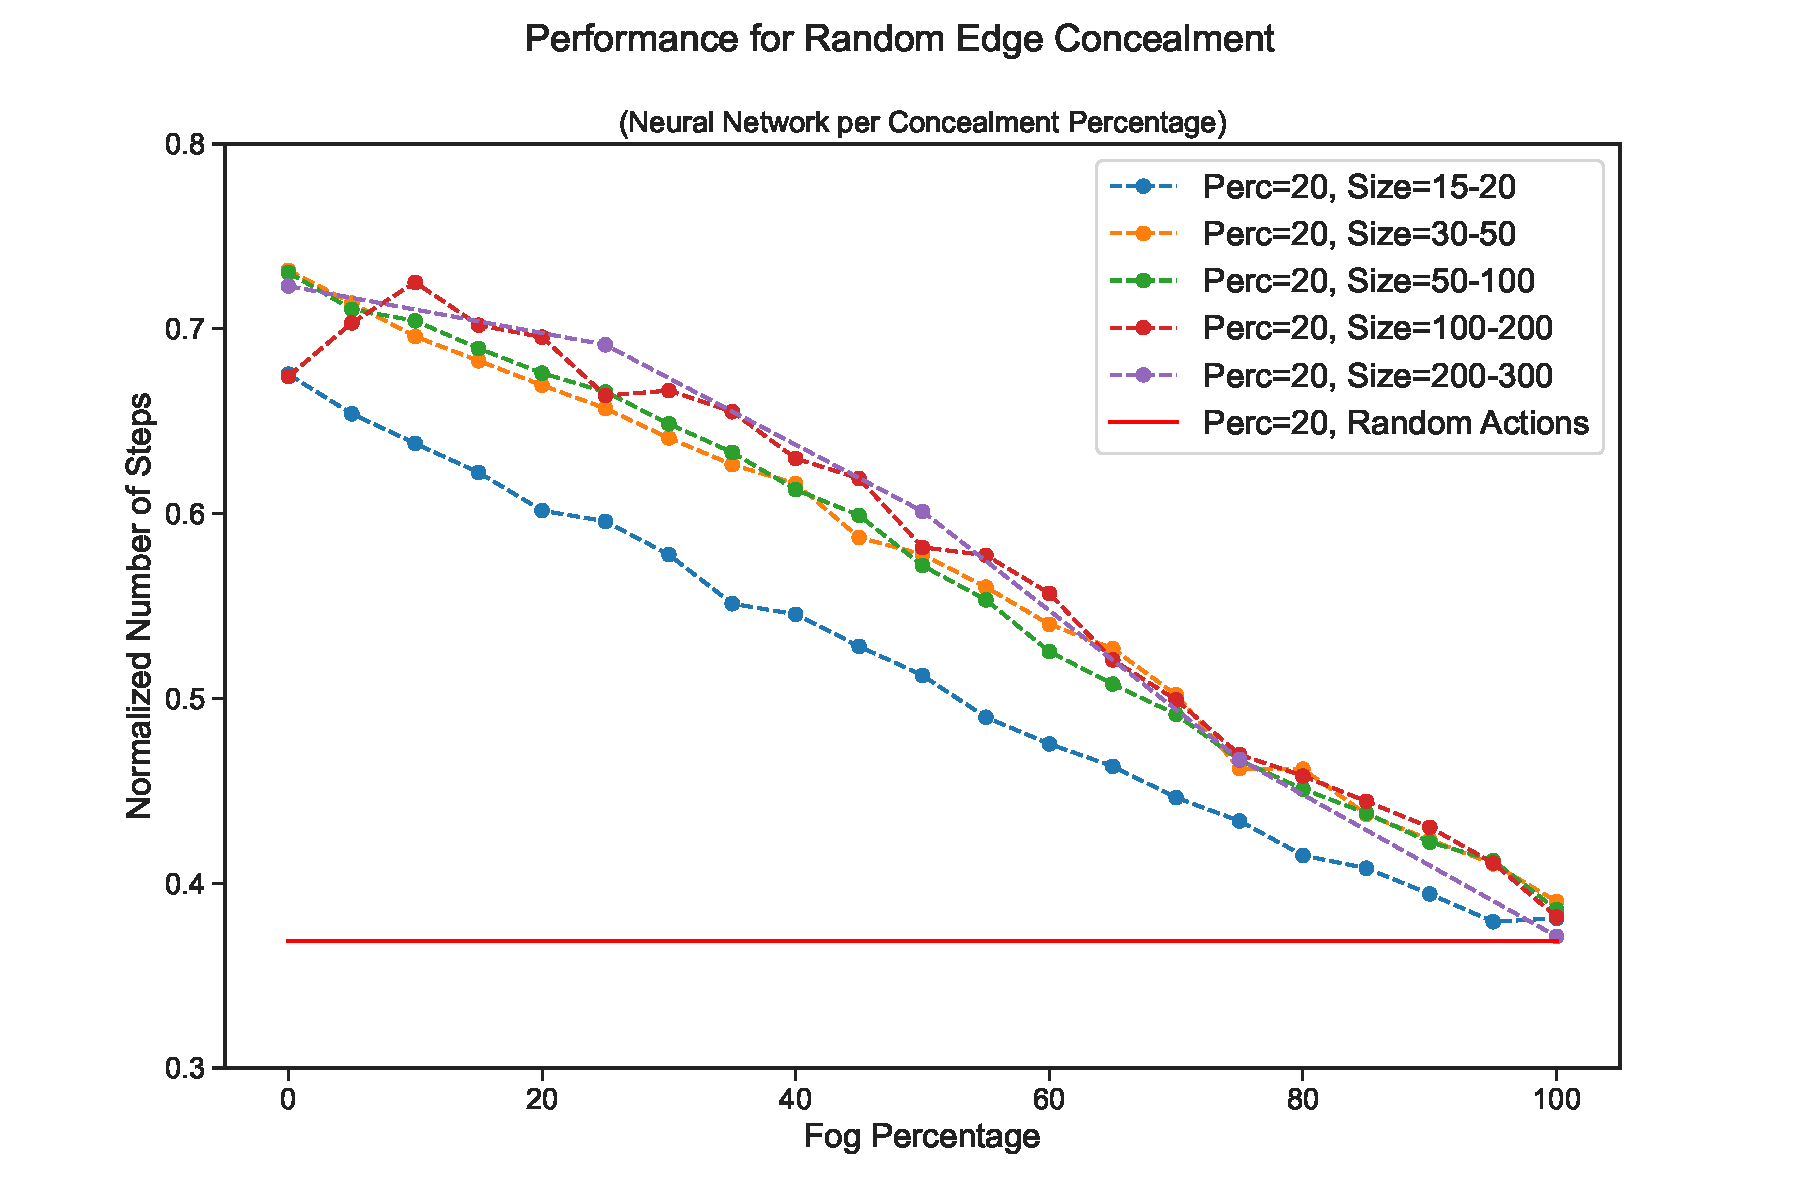
\includegraphics[scale=0.49]{Figures/percolation20_n200-300_k2-6_g2-3_random,all_fog.pdf}
    \caption[Caption Information]{\blindtext}
    \label{figure:random uniform (all models)}
\end{figure}

\begin{figure}[ht]
\sffamily\bfseries
    \centering
    % \textbf{Random Edge Concealment with Many Models}\par\medskip
    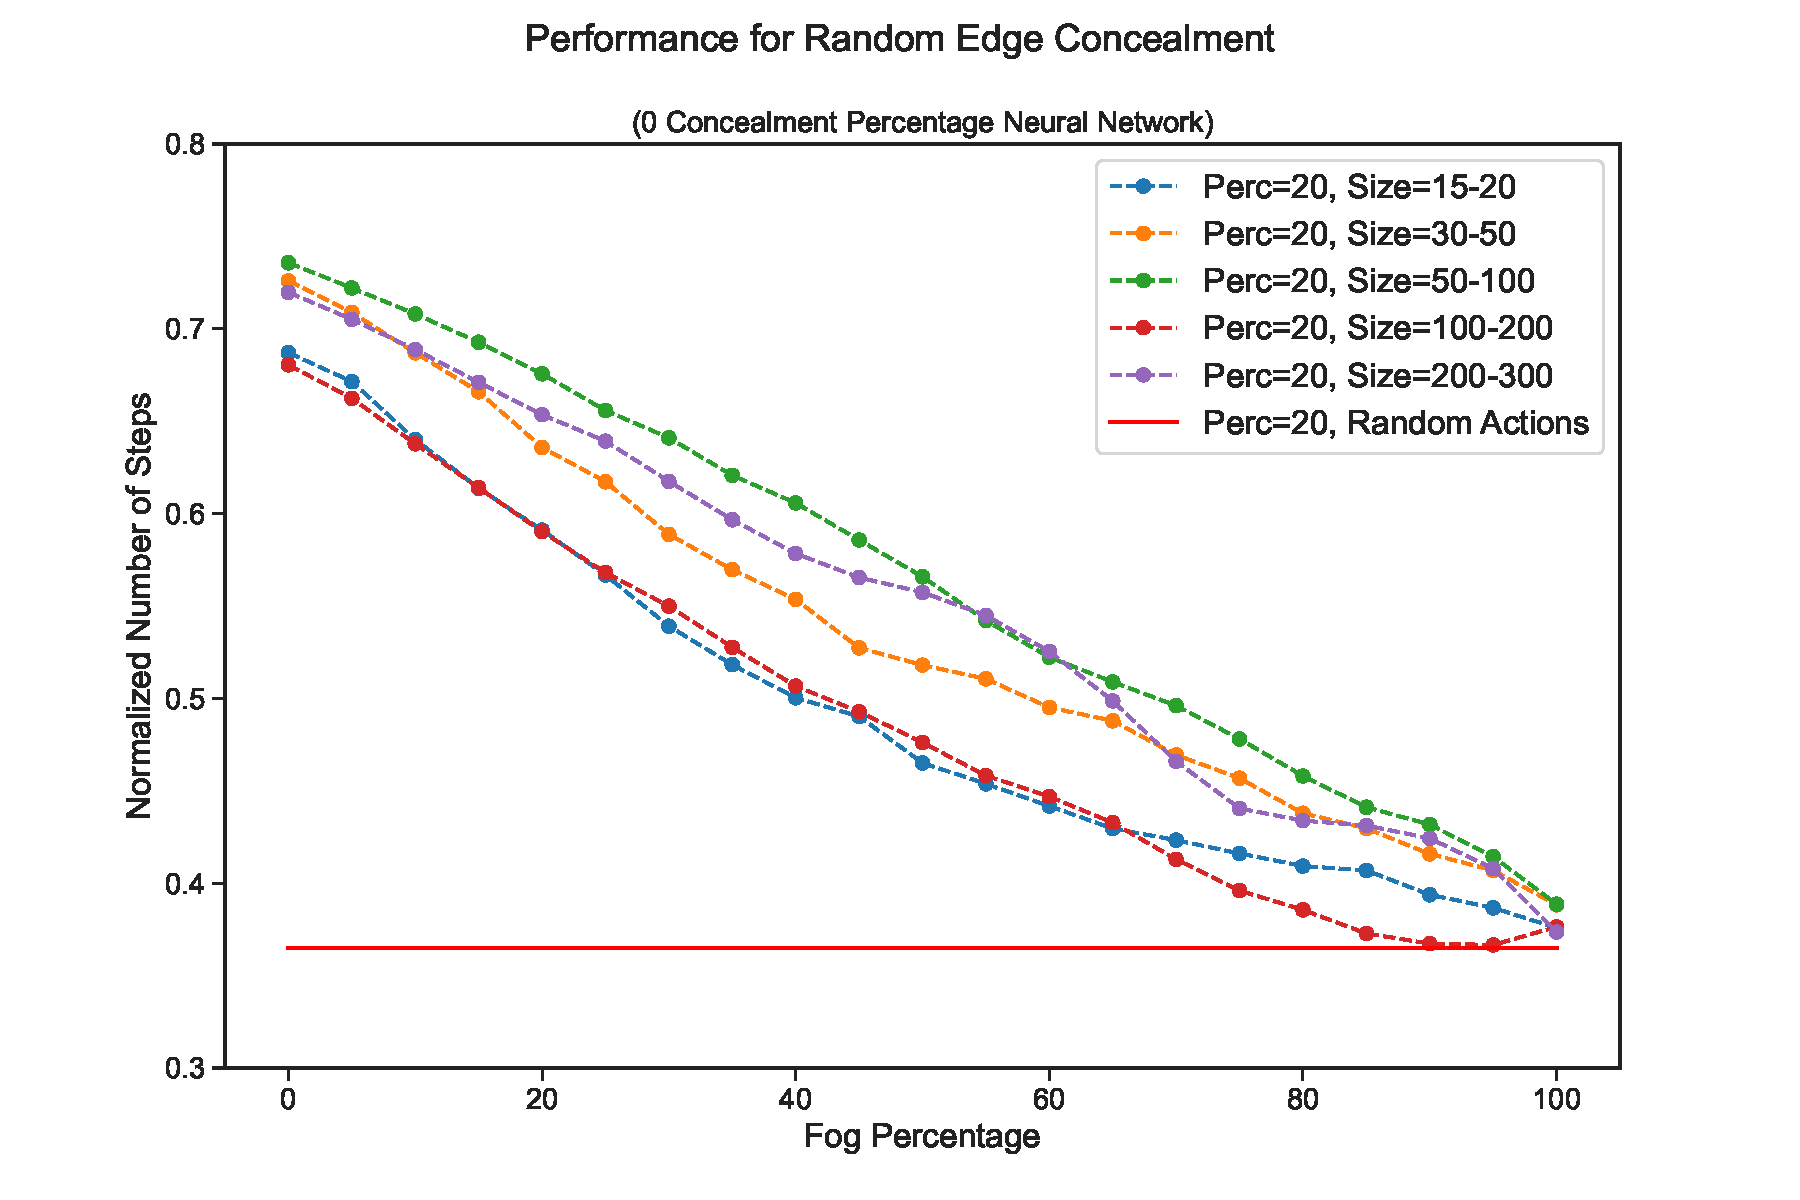
\includegraphics[scale=0.49]{Figures/percolation20_n200-300_k2-6_g2-3_p0.0_random,constant_fog.pdf}
    \caption[Caption Information]{\blindtext}
    \label{figure:random uniform (0 model)}
\end{figure}

\FloatBarrier
\clearpage
\subsection{Tabulated Performances}
% Random Edge Concealment
\begin{table}[ht]
    \centering \footnotesize
    \begin{tabular}{||c | c c ||} 
        \hline
        Network Size & \hyperref[figure:random uniform (all models)]{Area (All Models)} & \hyperref[figure:random uniform (0 model)]{Area (0.0 Model)}\\ [0.5ex] 
        \hline\hline
        15-20 & \gradient{0.13275} & \gradient{0.12930} \\ 
        \hline
        30-50 & \gradient{0.18738} & \gradient{0.17184} \\
        \hline
        50-100 & \gradient{0.18663} & \gradient{0.20129} \\
        \hline
        100-200 & \gradient{0.20822} & \gradient{0.12452} \\
        \hline
        200-300 & \gradient{0.20805}$\ast$ & \gradient{0.18448} \\ [1ex] 
        \hline
    \end{tabular}
    \caption[Caption information]{\blindtext}
    \label{table:uniform random}
\end{table}